In the current section we present the SALSA SCPool. We first show the data structures of SALSA in Section~\ref{alg-structure}, and then present the basic algorithm without stealing support in Section~\ref{alg-overview}. The stealing procedure is described in Section~\ref{alg-stealing}. The role of the chunk pools is shown in Section~\ref{alg-pools}, finally, we argue that SALSA is lock-free in Section~\ref{alg-properties}. 

\subsection{SALSA Structure\label{alg-structure}}
\newcounter{alg:non-fifo:lines}
\begin{algo}[!ht]
\caption{SALSA implementation of SCPool: Data Structures.} 
\label{alg:non-fifo-ds}
\scriptsize
\begin{minipage}[t]{0.48\textwidth}
\begin{distribalgo}[1]
\smallskip

\INDENT {{\bf Chunk type}}
	\STATE Task[CHUNK\_SIZE] tasks 
  \STATE int owner \comment {owner's consumer id}
\ENDINDENT

\INDENT {{\bf Node type}}
  \STATE Chunk c; initially $\bot$
  \STATE int idx; initially -1
  \STATE Node next; 
\ENDINDENT

\setcounter{alg:non-fifo:lines}{\value{ALC@line}} % store the line number
\end{distribalgo}
\end{minipage}%
%
\hfill
%
\begin{minipage}[t]{0.48\textwidth}
%
\begin{distribalgo}[1]
\setcounter{ALC@line}{\value{alg:non-fifo:lines}}
\smallskip

\INDENT {{\bf SALSA per consumer data structure}:}
  \STATE int consumerId
  \STATE List\tup{Node}[] chunkLists \comment {one list per producer + extra list for stealing (every list is single-writer multi-reader)} 
  \STATE Queue\tup{Chunk} chunkPool \comment {pool of spare chunks}
  \STATE Node currentNode, initially $\bot$ \comment {current node to work with} 
\ENDINDENT

\setcounter{alg:non-fifo:lines}{\value{ALC@line}}
\end{distribalgo}
\end{minipage}
\end{algo}


\begin{figure}[htb]
	\centering
	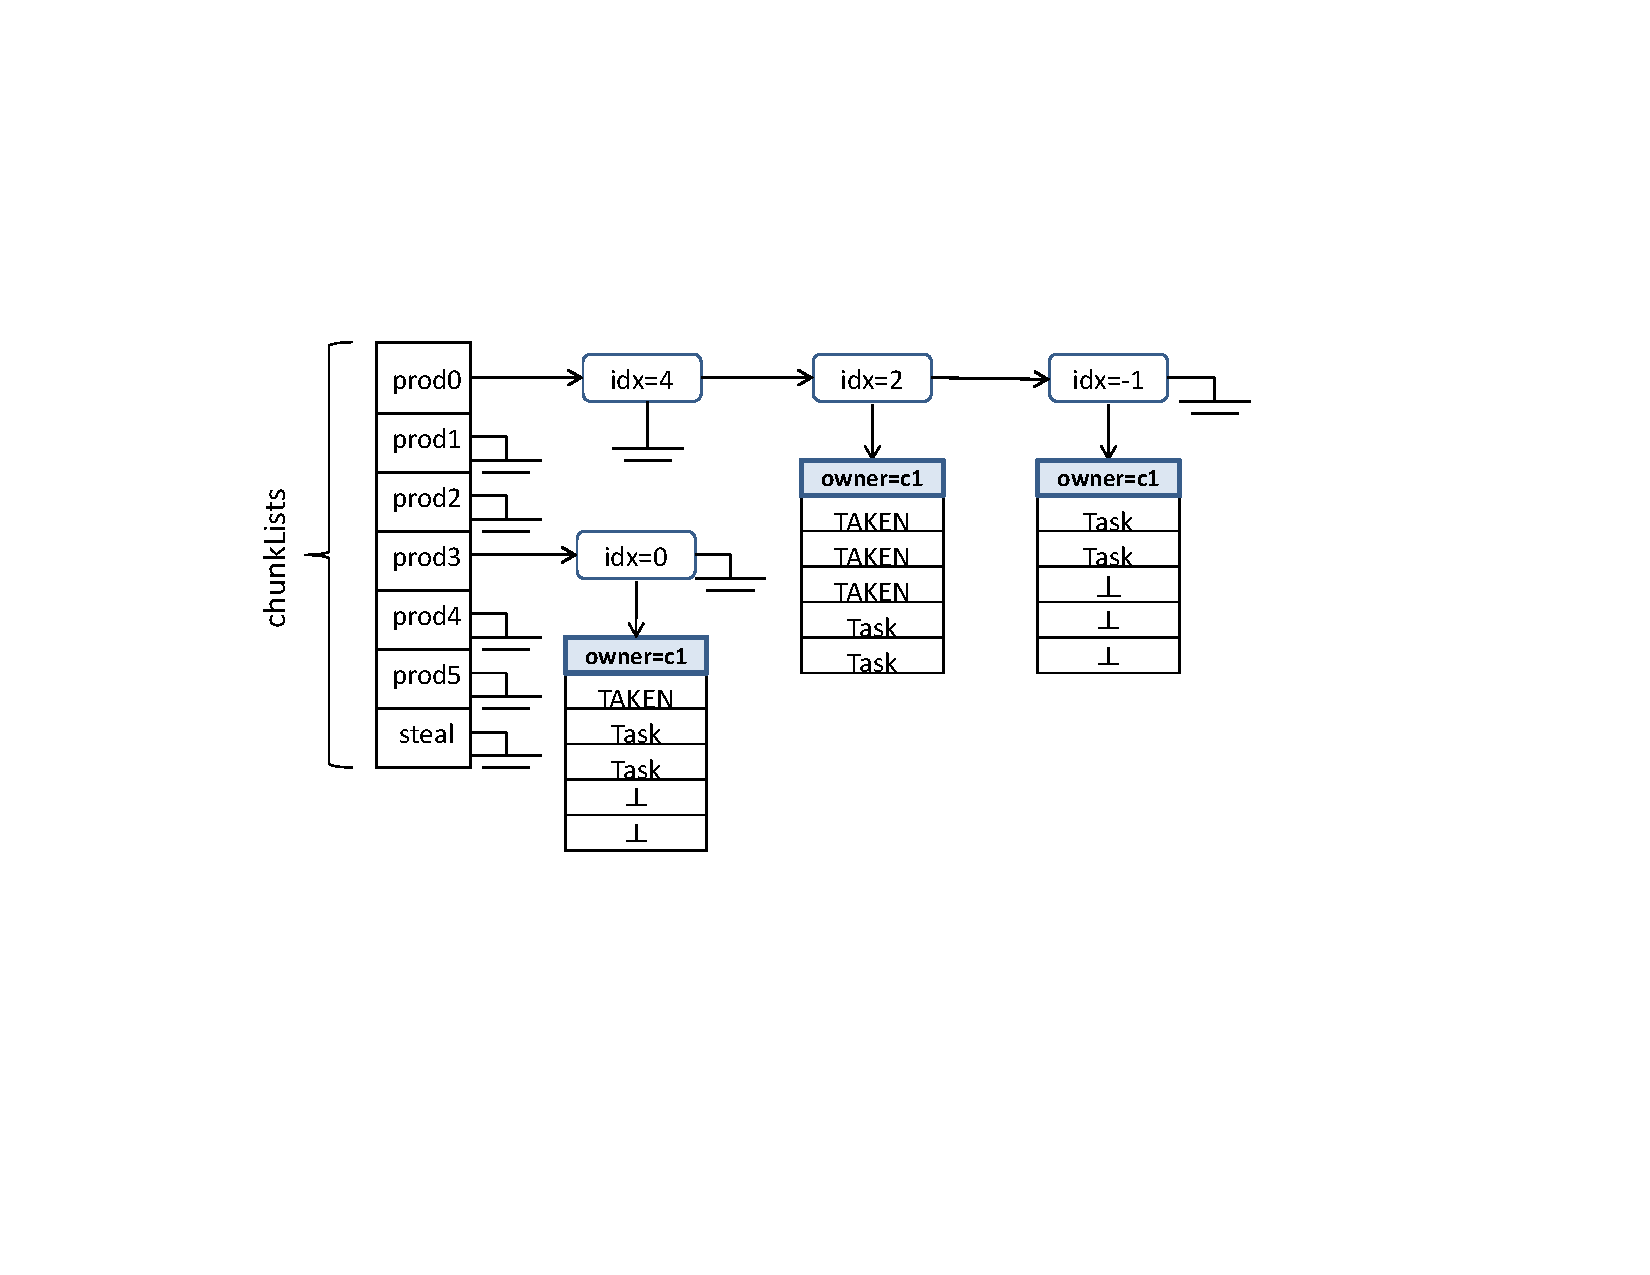
\includegraphics[height=0.3\textwidth]{figures/salsa-struct}
	\caption{
	    \footnotesize{Chunk lists in SALSA single consumer pool implementation. Tasks are kept in chunks, which are 
	    organized in per-producer lists; an additional list is reserved for stealing. Each list can be modified 
	    by the corresponding producer only. The only process that is allowed to retrieve tasks from a chunk is 
	    the owner of that chunk (defined by the ownership flag). A Node's index corresponds to the latest task taken from the chunk
	    or the task that is about to be taken by the current chunk owner. 
	    }}
	\label{fig:salsa-struct}
\end{figure}

We describe the implementation of a SALSA SCPool of some consumer $c_i$.
Its data structures are described in Algorithm~\ref{alg:non-fifo-ds} and partially depicted in Figure~\ref{fig:salsa-struct}. The tasks inserted to SALSA are kept in chunks, which are organized in per-producer chunk lists. Only the producer mapped to a given list can insert a task to any chunk in that list. Every chunk is owned by a single consumer whose id is kept in the \emph{owner} field of the chunk.
The owner is the only process that is allowed to take tasks from the chunk; if another process wants to take a task from the chunk, it should first steal the chunk and change its ownership. The owner of a chunk
residing at $c_i$'s SCPool is $c_i$ itself, unless that chunk is being stolen. A task entry in a chunk is used at most once. It holds the value $\bot$ initially, and TAKEN after the task it held has been consumed.

The per-producer chunk lists are kept in the array \emph{chunkLists} (see Figure~\ref{fig:salsa-struct}), where \emph{chunkLists[j]} keeps a list of chunks with tasks inserted by producer $p_j$. In addition, the array has a special entry \emph{chunkLists[steal]}, holding chunks stolen by $c_i$. Every list has a single writer who can modify the list structure (add or remove nodes), \emph{chunkLists[j]} can be modified only by the producer $p_j$, while the list \emph{chunkLists[steal]} can be modified only by the SCPool's owner $c_i$. Specifically, a consumed node (whose chunk was removed by the consumer) is lazily reclaimed and removed by the list's owner (typically a producer). For brevity, this is omitted from the pseudo-code bellow. Having a single writer allows us to implement the lists without synchronization primitives, similarly to the single-writer linked-list in~\cite{Michael:2004:HPS:987524.987595}.

In addition to the chunk pointer, each node keeps the index of the latest taken task. As we show in Section~\ref{alg-stealing}, this index plays a crucial role in chunk stealing. Safe memory reclamation is provided by using hazard pointers~\cite{Michael:2004:HPS:987524.987595} both for nodes and for chunks.

The free (reclaimed) chunks in SALSA are kept inside the SCPools in \emph{chunkPool}, a lock-free queue~\cite{Michael:1996:SFP:248052.248106}. These pools serve two purposes. First, they enable efficient memory reuse. Second, as we show in Section~\ref{alg-pools}, managing per-consumer chunk pools is good for load balancing. 
\subsection{Basic algorithm\label{alg-overview}}




The local variables and algorithms of the producer appear in
Algorithm~\ref{alg:producer-non-fifo}. The producer's code is fairly simple, the producer first
attempt to add tasks to the chunks it previously used, if this is the first produce action or the
previous chunk was already filled, the producer will attempt to take a chunk from the chunk pool and
add it to its list on the pool of the given consumer. If the pool is empty the operation will fail
with a FULL message, if produceForce was called the operation will not fail, instead a new chunk
will be allocated. 


\subsection{Stealing\label{alg-stealing}}
The stealing algorithm is presented in a function {\bf steal()} in Algorithm~\ref{alg:non-fifo}. 
We refer to the stealing consumer as $c_s$, the victim process whose chunk is being stolen is called $c_v$, and the stolen chunk is referred to as $ch$.

The idea is to turn $c_s$ to the exclusive consumer of $ch$, such that $s_c$ will be able to take tasks from the chunk without synchronization. 
In order to do that, $c_s$ changes the ownership of $ch$ (line~\ref{alg:line:chown}) and removes the chunk from the list of $c_v$ (line~\ref{alg:line:remove-chunk}). 
Once $c_v$ notices the change in the ownership it stops taking tasks from $ch$ (lines~\ref{alg:lines:stolen-chunk-end}--\ref{alg:lines:stolen-chunk-begin}). 

When the {\bf steal()} operation of $c_s$ occurs simultaneously with the {\bf takeTask()} operation of $c_v$, both $c_s$ and $c_v$ might try to retrieve the same task. Hence, $c_v$ notifies potential stealers of the task it is about to take by incrementing the \emph{idx} value of the $ch$'s node (line~\ref{alg:lines:ind-inc}). This value is later read by $c_s$ in line~\ref{alg:line:copy-prev-node} when creating a copy of $ch$'s node.

%Consider, for example, a scenario in which the $idx$ value is incremented from $10$ to $11$ during $c_v$'s {\bf takeTask()} operation.
Consider, for example, a scenario in which the $idx$ is incremented by $c_v$ from $10$ to $11$. 
If $c_v$ checks the ownership before it is changed by $c_s$, then $c_v$ takes the task at $11$ without synchronization (see line~\ref{alg:lines:fast-path}). Therefore, $c_s$ is never allowed to take a task pointed by \emph{idx}, and hence $c_v$ has to take the task at $11$ even if it observes the ownership change. 
After taking the chunk, $c_s$ will eventually try to take a task pointed by $idx+1$. However, if $c_s$ read $idx$ before it was incremented by $c_v$, $c_s$ might think that the value of $idx+1$ is $11$. In this case, both $c_s$ and $c_v$ will try to retrieve the task at $11$, hence both should use CAS operation in order to retrieve a task: line~\ref{alg:line:cas-steal} for $c_s$ and line~\ref{alg:line:cas-consumer} for $c_v$. 

The above algorithm works correctly as long as the stealing consumer can observe the node with the updated index value. 
This might not be a case if the same chunk is concurrently stolen by another consumer because the \emph{idx} of the original node would be obsolete. 
In order to prevent this situation, stealing a chunk from the pool of consumer $c_v$ is allowed only if $c_v$ is the owner of this chunk (line~\ref{alg:line:chown}). 

A naive way for $c_s$ to steal the chunk from $c_v$ would be first to change the ownership and then to move the chunk to the steal list. However, that would make our algorithm blocking because there exists a time that the chunk is unaccessible via the lists of $c_s$ and yet $c_s$ is its owner. In this case, as we explained above, the chunk cannot be stolen, which prevents taking the tasks from this chunk by other consumers. Therefore, our solution is to first add the original node to the steal list of $c_s$, change the ownership, and only then to replace the original node with a new node (lines~\ref{alg:line:resteal-begin}--\ref{alg:line:resteal-end}). 
 

% change the ownership (the consumer will check the ownership change)
% what about the first task retrieval? (the description includes the explanation about idx+1)
% what about concurrent stealing? (I want to see the updated idx value, the updated idx value is kept at node, hence I need to steal from the owner only)
% what about non-blocking properties? (want to allow others to always find a task...) 






% \paragraph{Stealing the chunk.} Before stealing a chunk, $c_1$ has to make sure $c_2$ will not take any more tasks from that chunk, so the $c_1$ may later take tasks with no need for synchronization. To achieve this $c_1$ must change the owner field of the chunk. Changing the ownership will prevent $c_2$ from taking tasks as a consumer always checks that he is the owner of the chunk before taking tasks. 
% 
% Before changing the ownership we must relate to two issues: (1) Stealing a chunk from the pool of consumer $c_2$ is allowed only if $c_2$ is the owner of the chunk that we steal, this is needed so it is guaranteed that $c_2$ reads the latest value of the idx, which is only found in the owner's node. (2) We want that other consumers would be able to steal the chunk during the process, so that the algorithm will stay lock-free. 
% 
% For those two reasons we must make the chunk accessible via $c_1$'s pool before changing ownership. However, we cannot simply add a new node to $c_1$'s steal list, as that node's idx field will not be updated if $c_2$ changes his idx field. Therefore, before changing ownership, $c_1$ adds $c_2$'s node to his steal list (Line~\ref{} in Algorithm~\ref{}). Now $c_1$ takes ownership (Line~\ref{}) and creates a new node with the updated idx that will replace the $c_2$'s node (Line~\ref{}), as the original idx may only change by one pending operation at most. Finally $c_1$ changes $c_2$'s node to point to NULL (Line~\ref{}) so that this node will not be used and will be lazily removed.
% 
% \paragraph{Taking the first task.} After the $c_1$ stole the chunk, he must attempt to take a task, so Property~\ref{steal-progress-property} will hold. $c_1$ will try to take the task at $idx+1$, however, this task may be also taken by $c_2$ if he started a consume operation before $c_1$ completed the node transfer. This is why $c_1$ must use a CAS operation to take this node (Line~\ref{}). $c_2$ must also attempt to take this node (Line~\ref{}) even if he noticed the ownership change, since he does not know if $c_1$ read the idx value before or after $c_2$ increased it Line~\ref{}.

% \vspace{5mm}\noindent
% We claim that the steal operation hold Property~\ref{steal-progress-property}. In line~\ref{} a chunk with at least one task is taken, therefore there is a task at $idx+1$. if $idx$ is updated during the stealing operation it means that the original consumer is taking that task and therefore the property holds. Otherwise, either the CAS in line~\ref{} failed and another consumer successfully stole the chunk and will return a task, or the current producer will reach line~\ref{}. In this line the CAS will be executed if the task wasn't already taken, and since either the stealing consumer or the original consumer will succeed performing the CAS.
\subsection{Chunk pools\label{alg-pools}}
As described in Section~\ref{alg-structure}, each consumer keeps a pool of free chunks.
When a producer needs a new chunk for adding a task to consumer $c_i$, it tries to get a chunk from $c_i$'s chunk pool -- if no free chunks are available, the {\bf produce()} operation fails.

As described in Section~\ref{sec:system}, our system-wide policy defines that if an insertion operation fails, then the producer tries to insert a task to other pools. Thus, the producer avoids adding tasks to overloaded consumers, which in turn decreases the amount of costly steal operations. 

Another SALSA property is that a chunk is returned to the pool of a consumer that retrieves the latest task of this chunk. 
Therefore, the size of the chunk pool of consumer $c_i$ is proportional to the rate of $c_i$'s task consumption.
This property is especially appealing for heterogeneous systems -- a faster consumer $c_i$ ", (e.g., one running on a stronger or less loaded core), will have a larger chunk pool, and so more {\bf produce()} operations will insert tasks to $c_i$, automatically balancing the overall system load. 

\subsection{SALSA safety}
\begin{figure}[htb]
	\centering
	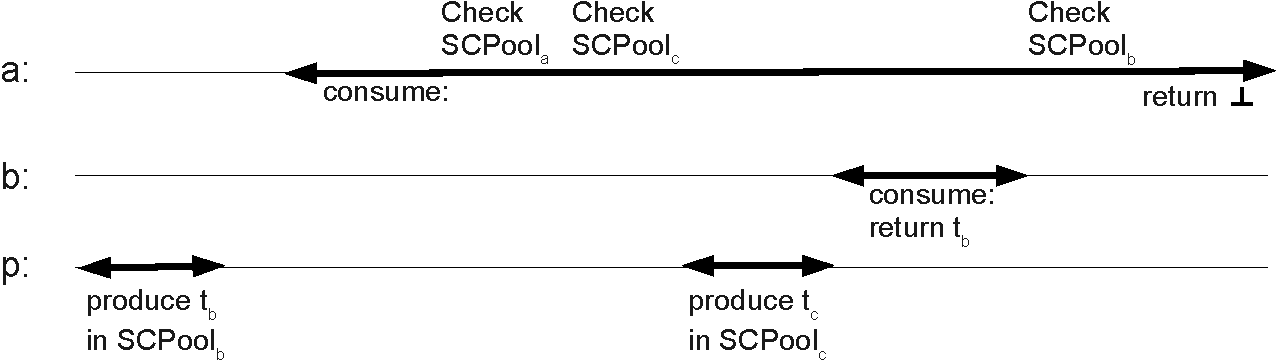
\includegraphics[width=0.7\textwidth]{figures/linearizability-example}
	\caption{\footnotesize{In this scenario $a$, $b$ and $c$ are the only consumers in the system and $p$ is the only producer. Above is a description of the following execution were $a$ trying to get a task: consumer $a$ fails to take a task from its own pool, and starts looking for chunks to steal in other pools. Assume that at this time there is a single non-empty chunk in the system, which is in $b$'s pool. Assume further that $a$ checks $c$'s pool before $b$'s pool and sees that it is empty. At this point a producer adds a task to $c$'s pool and then $b$ takes the last task from its pool before $a$ checks it. Thus, $a$ finds $b$'s pool to be empty, and returns $\bot$. There is no way to linearize this execution, because throughout the execution of the $a$'s operation, the system contained a task.}}
	\label{fig:linearizability-example}
\end{figure}

\paragraph{linearizability}
The algorithm as described in the previous sections is trivially wait-free as all operations of the SALSA pool always return, and the framework only calls a bounded number of those operations. However, this algorithm does not implement a linearizable task pool because an operation may return $\bot$ even when the pool is not empty. 

There are two possible reasons why a consumer may incorrectly return $\bot$. First, the consumer may ``miss'' one task added during its traversal, and another removed during the same traversal. Second, a consumer may miss a task in case a chunk is moved from one pool to another due to stealing. In order to identify these two cases, we add to each pool special counter \emph{emptyCount}, which is increased every time a chunk is reclaimed or stolen (i.e., every time a chunk is removed from the pool).
See the example in Figure~\ref{fig:linearizability-example}.

we now describe a way to make our algorithm linearizable which makes it only lock-free. 
We change the framework of section \ref{sec:system} so that a new function {\bf checkEmpty()} is called whenever a consumer fails to retrieve tasks from its pool and all other pools. This function ensures that $\bot$ is returned only if there is a time when there are no tasks in the system. If {\bf checkEmpty()} finds that the pool is not empty, the consumer restarts its operation. The {\bf checkEmpty()} function works as follows: the consumer traverses all the chunk lists of all SALSA pools in the system, to make sure that no tasks are present. After checking a pool, it reads its value of the \emph{emptyCount}. The consumer repeats this traversal $|consumers|$ times, where in all traversals except the first, it checks that the \emph{emptyCount} value is equal to the value it saw in the first traversal, i.e., that no chunks were moved during the traversal. The reason the consumer makes $|consumers|$ traversals is that other consumers may already stole or removed chunks but did not yet change \emph{emptyCount} and therefore their operations were not detected by the consumer. Since there may be up to $|consumers-1|$ pending operations by other consumers, it is guaranteed that after $|consumers|$ traversals in which no chunks were seen and the \emph{emptyCount} did not change, in one of the traversals the system contains no tasks, and therefore it is safe to return $\bot$. This method is similar to the one used in Concurrent Bags~\cite{Sundell:2011:LAC:1989493.1989550}. However, while our method requires a single fetch-and-increment operation per-steal and per-chunk, their operation requires an additional write on every produce operation, and a CAS operation for every empty chunk encountered in the traversal.

\paragraph{Lock-freedom}
This approach does not guarantee that a consumer will finish its operation. For example, in case the consumer's pool is empty, and its steal operation always fails, even when the system contains chunks, this consumer does not make progress. Nevertheless, the system is lock-free, i.e., there always exists some consumer that makes progress. Lock-freedom follows immediately from the following claim:


\begin{claim}
\label{claim:lock-free}
If a consumer fails in $c$ steal attempts from non-empty pools, where $c$ is the number of consumers in the system, then it is guaranteed that at least one consumer in the system returns a task during that time. 
\end{claim}
The proof for this claim is described in Appendix \ref{appendix:lock-freedom}.